\documentclass[12pt,twoside]{article}
\usepackage{MapsQt6Guis}
\usepackage{lscape}
%%\usepackage{stix}
\begin{document}
\hypersetup{
   pdfauthor     = {P. N. Daly},
   pdfsubject    = {MAPS Qt5/Qt6 GUIs Guide}
   pdftitle      = {MAPS Qt5/Qt6 GUIs Guide}
   pdfkeywords   = {MAPS Qt5/Qt6 GUIs Guide}
   }
\fancyhead[CE]{P.\ N.\ Daly}
\fancyhead[CO]{MAPS Qt5/Qt6 GUIs Guide}
\title{MAPS Qt5/Qt6 GUIs Guide}
\author{P.\ N.\ Daly}
\affil{Mountain Operations in Steward Observatory\altaffilmark{1} \\
933 N.\ Cherry Avenue, Tucson AZ 85719, U S A}
\altaffiltext{1}{
Steward Observatory is the research arm of the Department of Astronomy at the University of Arizona (UArizona). 
Its offices are located on the UArizona campus in Tucson, Arizona (US). Established in 1916, the first telescope 
and building were formally dedicated on April 23, 1923. It now operates, or is a partner in telescopes at five 
mountain-top locations in Arizona, one in New Mexico, one in Hawaii, and one in Chile. It has provided instruments 
for three different space telescopes and numerous terrestrial ones. Steward also has one of the few facilities in 
the world that can cast and figure the very large primary mirrors used in telescopes built in the early 21st century.}
\email{(520) 621-3648, pndaly@arizona.edu}
\begin{abstract}
This document describes the Qt5/Qt6 compliant GUIs associated with the MAPS project on the MMT.  \\
\end{abstract}

\tableofcontents
\listoffigures
%%\listoftables

\newpage
\section{Installation}
\label{Installation}

\subsection{Clone The GitHub Repository}
\label{Clone The GitHub Repository}

\noindent \emteal{git clone https://github.com/pndaly/MapsQt6Guis}

\noindent \emteal{cd MapsQt6Guis}

\subsection{Create A Virtual Environment (Optional)}
\label{Create A Virtual Environment (Optional)}

\noindent  \emteal{python3 -m venv .venv}

\noindent  \emteal{source .venv/bin/activate}

\noindent  \emteal{python3 -m pip install --upgrade pip}


\subsection{Install Dependencies}
\label{Install Dependencies}

Edit the {\tt requirements.txt} file to select a Qt version, then: \\

\noindent  \emteal{python3 -m pip install -r requirements.txt}

\section{Quick Start}
\label{Quick Start}

In the rest of this document, I assume you will be using Qt5. If you have upgraded to Qt6, replace `QT\_VERSION=5' with `QT\_VERSION=6'
in all subsequent commands. To get information on the status or control GUIs use: \\

\noindent \emteal{QT\_VERSION=5 python3 maps\_status\_gui.py --help} 

\noindent  \emteal{QT\_VERSION=5 python3 maps\_control\_gui.py --help}  \\

The command line arguments are: \\

\begin{description}
 \item[HOST] the \emph{indiserver} host machine, default=`localhost'
 \item[PORT] the \emph{indiserver} host machine port, default=7624
 \item[MODULE] the GUI module defined in the TAB\_DATA structure in {\tt maps\_indi.py}. The choices are
               \emph{all}, \emph{ao\_dm\_actuator}, \emph{ao\_dm\_admin}, \emph{ao\_dm\_housekeeper}, \emph{ao\_dm\_operate}, 
               \emph{ao\_logger}, \emph{chai2}, \emph{CyberPower}, \emph{Time}, \emph{Tcs}, \emph{Phil}, \emph{Amali} and \emph{New}, default=\emph{all}.
               Note that this is case-sensitive.
 \item[DELAY] the event loop delay period in ms, default=2000 (and see `Timing Loops' in section~\ref{Timing Loops} on page~\pageref{Timing Loops}).
 \item[ITEMS] the number of INDI streams to display (line-by-line) per page, default=25
 \item[FG] the foreground colour, default=\#FFFFFF (white)
 \item[BG] the background colour, default=\#000000 (black)
\end{description}


To select a specific GUI (for example `Phil'), just invoke it: \\

\noindent  \emteal{QT\_VERSION=5 python3 maps\_status\_gui.py --module=Phil \&}

\section{Status GUIs}
\label{Status GUIs}
\begin{figure}[!h]
 \centering
 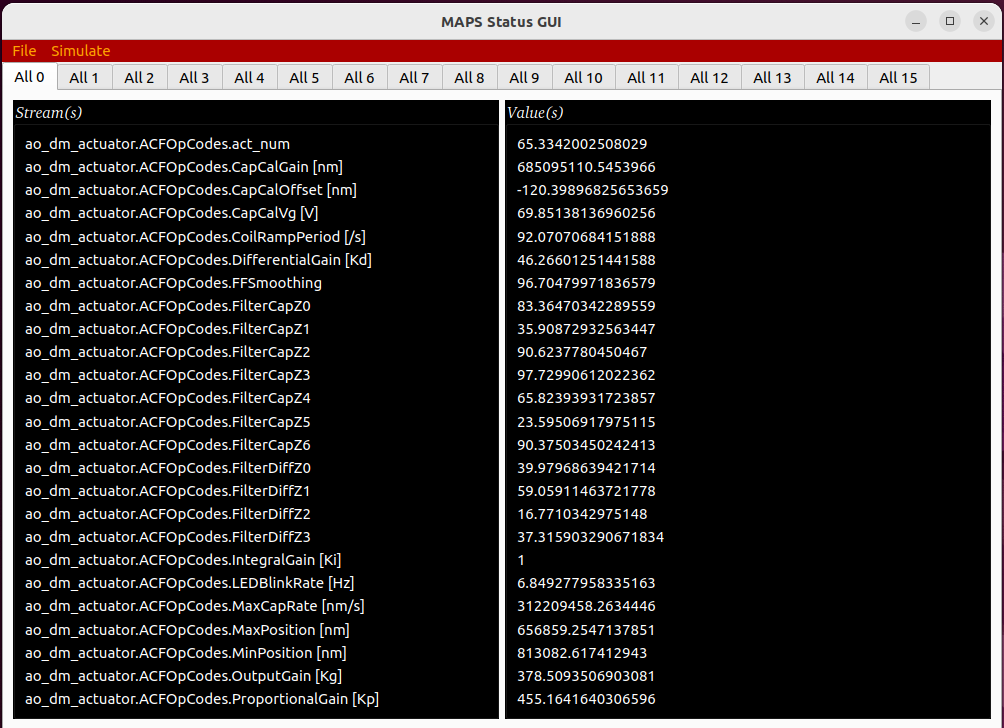
\includegraphics[width=0.5\linewidth]{MapsStatusGui.png}
 \caption{\sfmagenta{The `all' Status GUI. The LHS shows the INDI stream names or labels and the RHS the current values. The default is 15 items per page so these streams cover 16 tabs. Note the red/orange menubar colouring which indicates that simulation mode is enabled.}}
 \label{MapsStatusGui}
\end{figure}

The driving principle here is that \emph{anyone} can create their own customized status GUI
which does not allow \emph{any} control of INDI streams. Therefore, it is safe to do so.
It follows that this is the code that can build \emph{any} GUI it knows about as defined in {\tt maps\_indi.py}.
After following the steps outlined above, the GUI will be visible and can be run (here I choose the `all' module as
shown in figure~\ref{MapsStatusGui} on page~\pageref{MapsStatusGui}): \\

\noindent  \emteal{QT\_VERSION=5 python3 maps\_status\_gui.py --module=all \&} \\

\subsection{Running Multiple Status GUIs}
\label{Running Multiple Status GUIs}

\noindent  \emteal{QT\_VERSION=5 python3 maps\_status\_gui.py --module=Phil --items=40 \&}

\noindent  \emteal{QT\_VERSION=5 python3 maps\_status\_gui.py --module=Time \&}

\noindent  \emteal{QT\_VERSION=5 python3 maps\_status\_gui.py --module=CyberPower \&}

\noindent  \emteal{QT\_VERSION=5 python3 maps\_status\_gui.py --module=Amali \&}

\section{Control GUIs}
\label{Control GUIs}
\begin{figure}[!h]
 \centering
 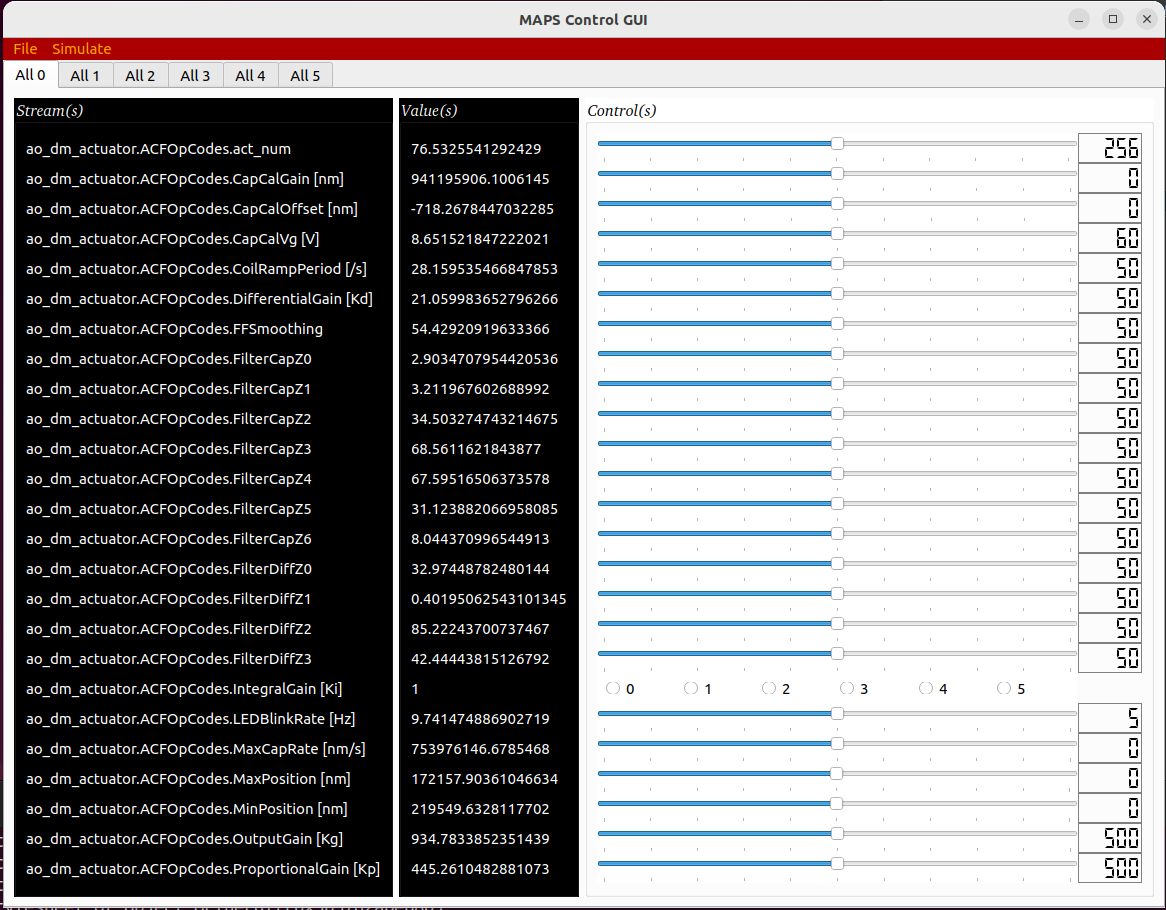
\includegraphics[width=0.5\linewidth]{MapsControlGui0.png}
 \caption{\sfmagenta{The `all' Control GUI. The LHSP shows the INDI stream names or labels and the CP the current values. 
  The default is 15 items per page so these streams cover 6 tabs since only a subset are write controllable. 
  Note the red/orange menubar colouring which indicates that simulation mode is enabled.
  The RHSP contains control widgets scaled to the datarange defined in {\tt maps\_indi.py} elminating the need for 
  error checking any inputs.}}
 \label{MapsControlGui0}
\end{figure}
\begin{figure}[!h]
 \centering
 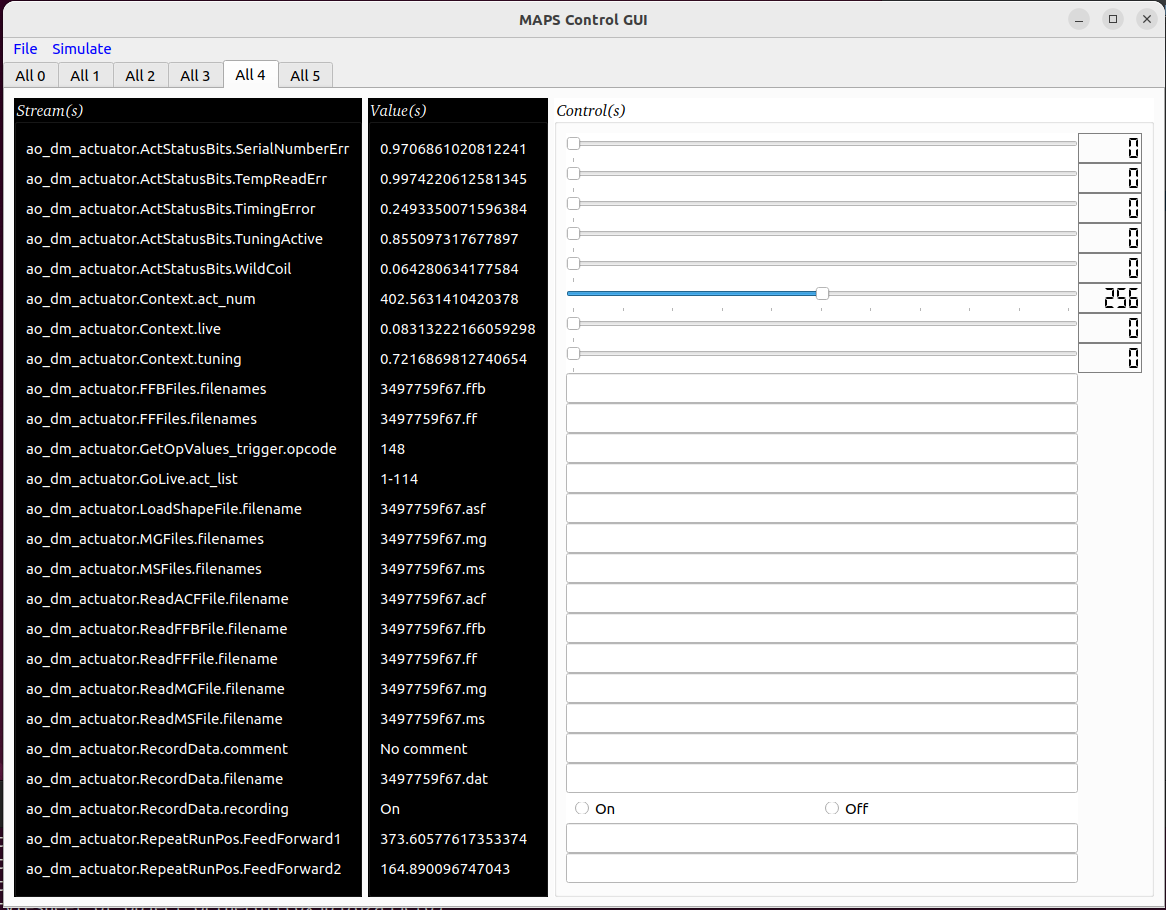
\includegraphics[width=0.5\linewidth]{MapsControlGui4.png}
 \caption{\sfmagenta{The `all' Control GUI. This shows a different tab in the same control GUI as above but
  the palegreen/blue menubar colouring which indicates that simulation mode is disabled.}}
 \label{MapsControlGui4}
\end{figure}
\begin{figure}[!h]
 \centering
 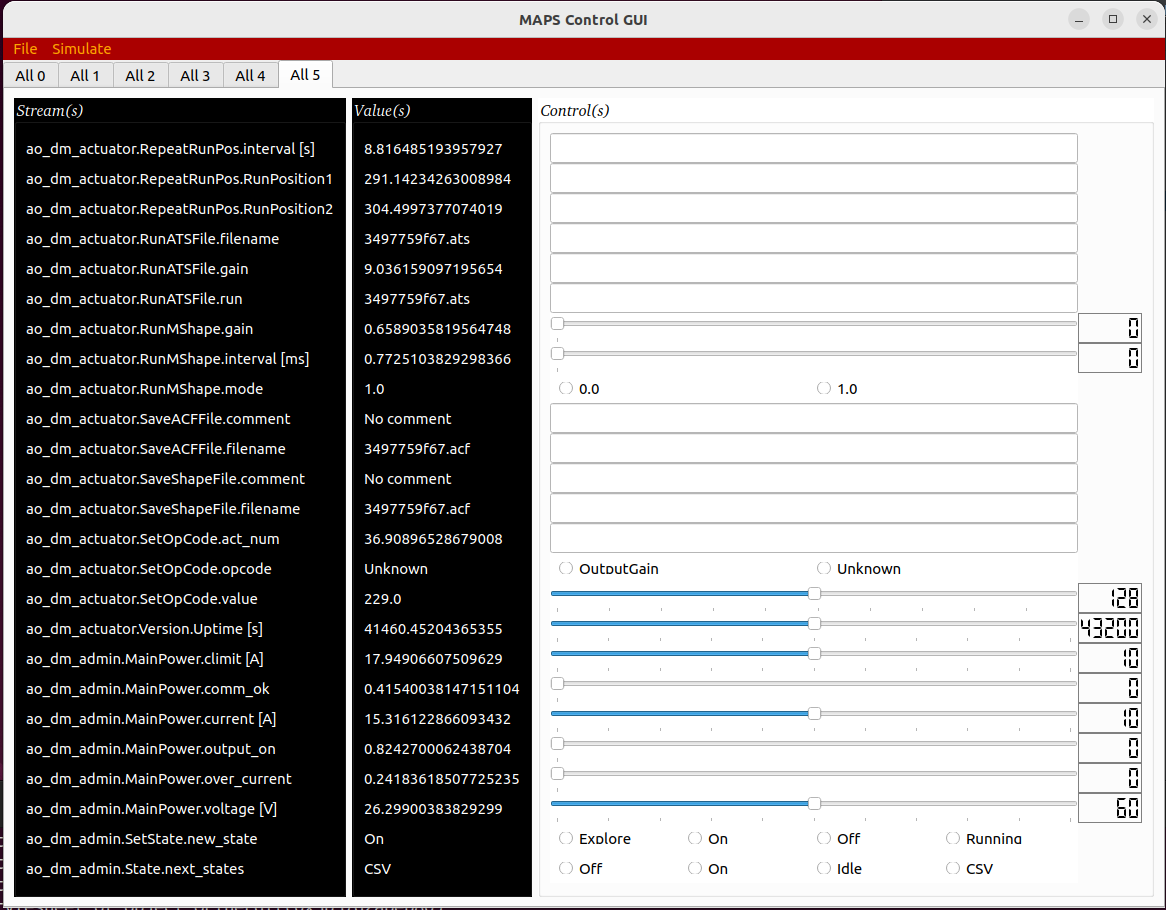
\includegraphics[width=0.5\linewidth]{MapsControlGui5.png}
 \caption{\sfmagenta{The `all' Control GUI. This shows a different tab in the same control GUI as above which displays entry widets as well as sliders and radio buttons.}}
 \label{MapsControlGui5}
\end{figure}

The driving principle here is that there should only be 1 point of control (but this is not currently
enforced and it is left to a future developer to add singleton class support). The method to add a new
control GUI is exactly the same as adding a new status GUI but the code will only create widgets whose
INDI streams are identified as `wo' (write-only) or 'rw' (read-write). If, for example, you try to run the `Phil'
control GUI, it will not produce any GUI control window but will return: \\

\noindent \emteal{QT\_VERSION=5 python3 maps\_control\_gui.py --module=Phil}\\
2024-07-15 15:40:01,288 line:133   No (writeable) controls selected\\

This is because all elements within the (pre-defined) `Phil' GUI are read only so not controllable.
However, the following command produces the output(s) shown in
figures~\ref{MapsControlGui0}, ~\ref{MapsControlGui4} and ~\ref{MapsControlGui5} on 
pages~\pageref{MapsControlGui0}, ~\pageref{MapsControlGui4} and ~\pageref{MapsControlGui5} respectively: \\

\noindent \emteal{QT\_VERSION=5 python3 maps\_control\_gui.py --module=all}\\

The design principle for \emph{MapsQt6Guis} control has 3 side-by-side panels: the left-hand-side panel (LHSP) shows the data
stream name, the central panel (CP) shows the current value and the right-hand-side panel (RHSP) contains the controls for submitting new
values. Note that the LHSP and CP are just a re-creation of the status GUI.

Note that the RHSP controls are preferable to the Maga-AO way of doing things which has a single
entry widget beneath the current value(s) list because:

\begin{enumerate}
 \item there is no risk of a typing error writing a valid value to an invalid stream (which could be dangerous);
 \item the control type and data limits are taken from the appropriate data structure in {\tt maps\_indi.py} so
       out-of-range values are avoided
  \emph{i.e. viz.,} there is no risk of an invalid value being written to a valid stream;
 \item thee utilization of datatype and datarange elements from the appropriate data structure element in {\tt maps\_indi.py}, means that
       no error checking is required saving lots of lines of code.
\end{enumerate}

\section{Adding New GUIs}
\label{Adding New GUIs}

The principal file for driving new GUI development is {\tt maps\_indi.py}. This
contains a set of data structures defining the INDI streams associated with each
sub-system. I have used the original Elwood Downey names but these are just placeholders
so can be renamed in future without loss of functionality. 
To add a new GUI, use the PND\_GUI as an exemplar. In {\tt maps\_indi.py}: \\

\begin{enumerate}
 \item Create the PND\_GUI structure;
 \item Add an entry to TAB\_NAMES providing a unique key (`Phil') and preferred tab name (``Phil's Shiny New GUI'');
 \item Add an entry to TAB\_DATA with the same key as the previous step (`Phil') and referencing the PND\_GUI data structure.
\end{enumerate}

That's it!

\section{Adding New INDI Streams}
\label{Adding New INDI Streams}
Adding new streams is as simple as defining a new data structure and including it in the flattened dictionary called
ALL\_STREAMS in {\tt maps\_indi.py}. For example, let us assume we have a new INDI stream called `telescope' and it has 3 ad-hoc data points:

\begin{description}
 \item[telescope.focus.value] this is `rw' so can be changed within the (known) range -275 through +290 microns;
 \item[telescope.truss.temperature] this is `ro' so cannot be changed;
 \item[telescope.primary.fan] this is `wo' and can only be toggled between 2 positions `Off' and `On'.
\end{description}

So, in the new dictionary each INDI stream is a separate key that contains a sub-dictionary with the following keys:

\begin{description}
 \item[actval] this is the actual value shown by the widget and can be received from INDI or simulated;
 \item[datarange] this is an appropriate data range. For floats it is typically a bounded tuple. For integers it can
    be a bounded tuple or a list. For strings, it can either be a string or a list of strings;
 \item[datatype] the data type. Supported datatypes are `float', `int' and `str'. There is a placeholder type called `binary'
    but this is not currently used (see section~\ref{Binary Large Objects and Redis} on page~\pageref{Binary Large Objects and Redis});
 \item[label] if specified, the label is used but if it is `None' a label is populated from the dictionary key;
 \item[permission] `ro' for read-only, `rw' for read-write or `wo' for write-only;
 \item[simval] the simulation value or function to be used to calculate one;
 \item[tooltip] a human-readable pop-up textual hint seen by hovering over the widget;
 \item[unit] the unit of the data, if there is one;
 \item[widget] defined as None and populated according to the datatype: `float' and `int' can generate sliders, `int' and `str' can
    generate radio buttons, `str' can generate entry widgets (on the fly).
\end{description}

So, the new dictionary in {\tt maps\_indi.py} would look like this:

\begin{verbatim}
TELESCOPE = {
 "telescope.focus.value": {
    "actval": math.nan,
    "datarange": (-275.0, 290.0),
    "datatype": "float",
    "label": "Telescope Focus",
    "permission": "rw",
    "simval": random.uniform,
    "tooltip": "Telescope focus via the Galil controller",
    "unit": "micron",
    "widget": None,
 },
 "telescope.truss.temperature": {
    "actval": math.nan,
    "datarange": (-25.0, 75.0),
    "datatype": "float",
    "label": None,
    "permission": "rw",
    "simval": random.uniform,
    "tooltip": "Telescope truss temperature",
    "unit": "Celsius",
    "widget": None,
 },
 "telescope.primary.fan": {
    "actval": "Off",
    "datarange": ["On", "Off"],
    "datatype": "str",
    "label": None,
    "permission": "wo",
    "simval": random.choice,
    "tooltip": "Toggle the primary air-blowing fan off or on",
    "unit": "",
    "widget": None,
 },
}
\end{verbatim}

We then replace:\\ 

\noindent \small{ALL\_STREAMS = \{**\{\}, **AO\_DM\_ACTUATOR, **AO\_DM\_ADMIN, **AO\_DM\_HOUSEKEEPER, **AO\_OPERATE, **AO\_LOGGER, **CHAI2, **CYBER\_POWER, **TIME, **TCS\}} \\

with \\

\noindent \small{ALL\_STREAMS = \{**\{\}, **AO\_DM\_ACTUATOR, **AO\_DM\_ADMIN, **AO\_DM\_HOUSEKEEPER, **AO\_OPERATE, **AO\_LOGGER, **CHAI2, **CYBER\_POWER, **TIME, **TCS, **TELESCOPE\}} \\

When we edit the {\tt maps\_indi.py} file we should always check for data consistency by executing the command: \\

\noindent  \emteal{python3 maps\_indi.py} \\

If it returns an error, please correct it before proceeding with any other development. If it does not return an error, 
we are done and free to use the new INDI streams in the GUIs.
 
\section{Other Considerations}
\label{Other Considerations}

\subsection{A Generic Solution}
\label{A Generic Solution}
As can be seen, the solution provided is totally generic and relies only on the data within the various dictionaries
in  {\tt maps\_indi.py} being reviewed and kept up-to-date and accurate.

\subsection{Simulation Mode}
\label{Simulation Mode}
Note that there is a simulation mode enabled at this time to allow software developers or curious users to 
run the code without the \emph{indiserver} being present. This facility can be toggled on and off
but you should \emph{not} assume that turning simulation off automatically connects the code to the
\emph{indiserver}. It does not. It is also possible that this simulation mode behaviour will be changed
in a future release (including its removal when its utility is no longer valid).

So, to fully connect to the \emph{indiserver}, turn `simulate' off and then use the file menu `Connect' item
as shown in figure~\ref{FileMenu} on page~\pageref{FileMenu}. The keyboard shortcut is `Ctrl+C'.

Finally, note that if the connection to the \emph{indiserver} fails, the GUI will \emph{automatically}
re-enable simulation mode!

\subsection{Log Files}
\label{Log Files}
Log files are created in {\tt /tmp/maps\_status\_gui.log} and {\tt /tmp/maps\_control\_gui.log}.

\subsection{Control GUI}
\label{Control GUI}
The control GUI should be a \emph{singleton} class and, currently, it is not.

\subsection{Binary Large Objects and Redis}
\label{Binary Large Objects and Redis}

At the present time, the code does not handle binary large objects (BLOBs) nor does it handle \emph{redis} publish-subscribe
data streams. The former needs thinking about but the latter should be pretty straightforward given the infrastructure code
developed here.

\subsection{Timing Loops}
\label{Timing Loops}
INDI is a publish-subscribe paradigm mechanism and as such relies on `asynchronous i/o'. GUIs, in order to remain responsive to
mouse clicks and the like, use the `event driven' paradigm. These two are not necessarily compatible so may not play well together: 
there is the possibility of a system lock and/or race condition. In the code, I have provided the `--delay' command line argument to 
adjust one of these loops so that responsiveness and timely updates can peacefully coexist. This delay may well be different for the 
different GUI modules defined and can only be determined empirically.

\appendix
\section{Miscellaneous Screenshots}
\label{Miscellaneous Screenshots}
\begin{figure}[!h]
 \centering
 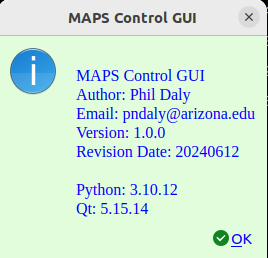
\includegraphics[width=0.25\linewidth]{AboutBox.png}
 \caption{\sfmagenta{Rudimentary information on the software is included in the `About' box.}}
 \label{AboutBox}
\end{figure}

\begin{figure}[!h]
 \centering
 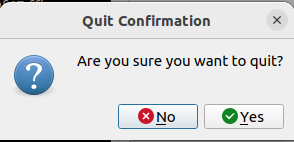
\includegraphics[width=0.25\linewidth]{QuitBox.png}
 \caption{\sfmagenta{When you exit the GUI, you will be prompted to confirm your decision.}}
 \label{QuitBox}
\end{figure}

\begin{figure}[!h]
 \centering
 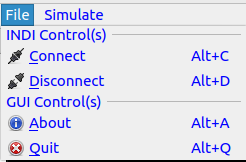
\includegraphics[width=0.25\linewidth]{FileMenu.png}
 \caption{\sfmagenta{The `Filemenu' contains connect and disconnect buttons plus the `About' and `Quit' controls.}}
 \label{FileMenu}
\end{figure}


\end{document}
